\textbf{Ejemplo 3}\\

Supongamos que hay en estudio dos opciones de inversión: el proyecto A que requiere una inversión inicial de 200.000 COP y produce un ingreso de 31.160 COP durante 10 períodos y el proyecto B que tiene un costo de  100.000 COP y produce un ingreso durante 10 períodos de 16.280 COP. Se tiene una tasa de oportunidad del 5\% período mes vencido. Determinar cual es el mejor proyecto.
\\

\textbf{Solución.}\\
%La tabla ira centrada
\begin{center}
	\renewcommand{\arraystretch}{1.5}% Margenes de las celdas
	%Creación de la cuadricula de 3 columnas
	\begin{longtable}[H]{|c|c|c|}
		%Creamos una linea horizontal
		\hline
		%Definimos el color de la primera fila
		\rowcolor[HTML]{FFB183}
		%%%%% INICIO ASIGNACIÓN PERÍODO FOCAL %%%%%%%
		%%%%%%%%%% INICIO TITULO
		%Lo que se hace aquí es mezclar las 3 columnas en una sola
		\multicolumn{3}{|c|}{\cellcolor[HTML]{FFB183}\textbf{1. Asignación período focal}}                                                            \\ \hline
		%%%%%%%%%% FIN TITULO
		%%%%% INICIO DECLARACIÓN DE VARIABLES %%%%%%%
		\multicolumn{3}{|c|}{$pf : 0 pmv$}                                                                                                            \\ \hline

		%%%%%%%%%%% INICIO TITULO
		\rowcolor[HTML]{FFB183}
		\multicolumn{3}{|c|}{\cellcolor[HTML]{FFB183}\textbf{2. Declaración de variables}}                                                            \\ \hline
		%%%%%%%%%%% FIN TITULO
		%%%%%%%%%%% INICIO MATEMÁTICAS

		$\textbf{Proyecto A}$                                      & \multicolumn{2}{c|}{$ \textbf{Proyecto B} $}                                     \\
		$i = TIO = 5\% $ $ pmv  \hspace{0.3cm} $                   & \multicolumn{2}{c|}{$ i  = TIO  = 5\% pmv$}                                      \\
		$ n = 10 pmv $                                             & \multicolumn{2}{c|}{ $ n = 10 pmv $ }                                            \\
		$\text{Inversión inicial} = 200\text{.}000$ $COP $         & \multicolumn{2}{c|}{ $ \text{Inversión inicial} =  100\text{.}000$ $COP$}        \\
		$ \text{Ingreso por 10 periodos} =  31\text{.}160$ $ COP $ & \multicolumn{2}{c|}{ $ \text{Ingreso por 10 periodos} = 16\text{.}280$ $ COP $ }
		\\
		$  $                                                       & \multicolumn{2}{c|}{ $ $ }
		\\
		\hline
		%%%%%%%%%% FIN MATEMÁTICAS
		%%%%% INICIO FLUJO DE CAJA
		\rowcolor[HTML]{FFB183}
		\multicolumn{3}{|c|}{\cellcolor[HTML]{FFB183}\textbf{3. Diagrama de flujo de caja}}                                                           \\ \hline
		%Mezclamos 3 columnas y pondremos el dibujo
		%%%%%%%%%%%%% INSERCIÓN DE LA IMAGEN
		%Deberán descargar las imágenes respectivas del drive y pegarlas en la carpeta
		%n_capitulo/img/ejemplos/1/capitulo1ejemplo1.pdf  (el /1/ es el numero del ejemplo)
		\multicolumn{3}{|c|}{ 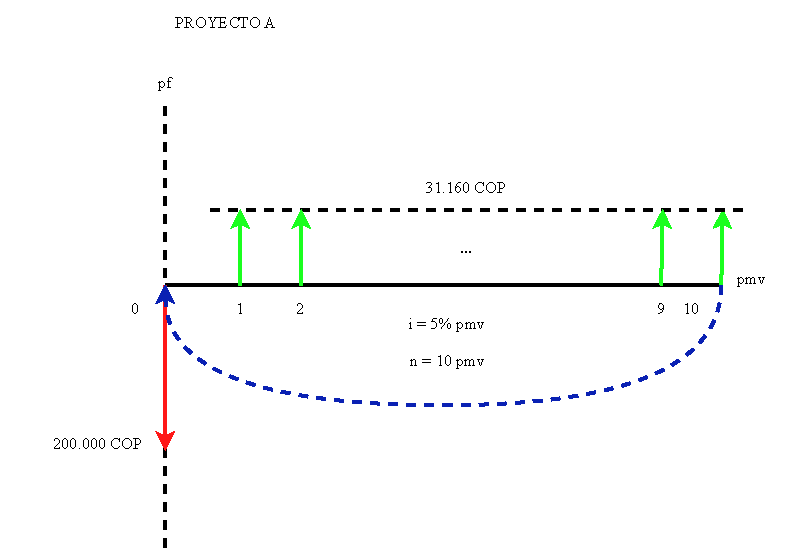
\includegraphics[scale=1]{ejemplos/3/Graf1Ej3Cap11.pdf} }
		\\
		\multicolumn{3}{|c|}{ 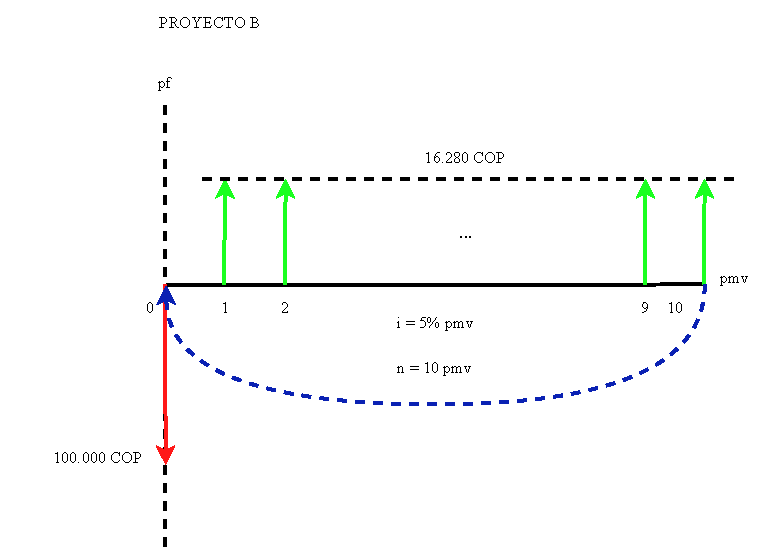
\includegraphics[scale=1]{ejemplos/3/Graf2Ej3Cap11.pdf} }
		\\\hline
		%%%%%%%%%%%%% FIN INSERCIÓN DE IMAGEN
		%%%%%FIN FLUJO DE CAJA



		%%%%% INICIO DECLARACIÓN FORMULAS
		%%%%%%%%%%% INICIO TITULO
		\rowcolor[HTML]{FFB183}
		\multicolumn{3}{|c|}{\cellcolor[HTML]{FFB183}\textbf{4. Declaración de fórmulas}}                                                             \\ \hline
		%%%%%%%%%%% FIN TITULO
		%%%%%%%%%%% INICIO MATEMÁTICAS
		\multicolumn{3}{|c|} {VPN =	$\sum F_{n}(1+i)^{-n}$   Valor presente neto.}                                                                    \\ \hline

		%%%%%%%%%% FIN MATEMÁTICAS
		%%%%%% INICIO DESARROLLO MATEMÁTICO
		\rowcolor[HTML]{FFB183}
		%%%%%%%%%%INICIO TITULO
		\multicolumn{3}{|c|}{\cellcolor[HTML]{FFB183}\textbf{5. Desarrollo matemático}}                                                               \\ \hline
		%%%%%%%%%% FIN TITULO
		%%%%%%%%%% INICIO MATEMÁTICAS
		\multicolumn{3}{|c|}{$ VPN(A)=- 200\text{.}000 COP + 31\text{.}160 COP(\frac{1-(1+0.05)^{-10}}{0.05})= $ $ 40\text{.}609,26 COP$}
		\\

		\multicolumn{3}{|c|}{$ VPN(B)=- 100\text{.}000 COP + 16\text{.}280 COP(\frac{1-(1+0.05)^{-10}}{0.05})=$ $ 25\text{.}709,84 COP$}
		\\\hline
		\multicolumn{3}{|c|}{$ \textbf{El VPN nos dice que es mejor el proyecto A}$}
		\\
		\multicolumn{3}{|c|}{$ \textbf{Evaluando el TIR}$}
		\\
		\multicolumn{3}{|c|}{$ TIR(A) = -200\text{.}000 COP + 31\text{.}160 COP(\frac{1-(1+i)^{-10}}{0.05})= $ $ 0 COP$}
		\\
		\multicolumn{3}{|c|}{$ \text{Calculando i por interpolación se tiene que TIR(A)=9\% pmv} $}
		\\
		\multicolumn{3}{|c|}{$ TIR(B)=- 100\text{.}000 COP + 16\text{.}280 COP(\frac{1-(1+i)^{-10}}{0.05}) = $ $ 0 COP$}
		\\
		\multicolumn{3}{|c|}{$ \text{Calculando i por interpolación se tiene que TIR(B)=10,01\% pmv} $}
		\\
		\multicolumn{3}{|c|}{$ \text{La TIR nos dice que es mejor el proyecto B, lo cual contradice al VPN.} $}
		\\
		\multicolumn{3}{|c|}{$ \text{Intentamos aclarar esta contradicción usando la TIRM.} $}
		\\
		\multicolumn{3}{|c|}{$ \textbf{Evaluando la TIRM } $}
		\\
		\multicolumn{3}{|c|}{$ \text{TIRM(A):  Trasladamos a valor final la serie de 10 ingresos de 31.160 COP y tenemos:} $}
		\\
		\multicolumn{3}{|c|}{$ 31\text{.}160 COP(\frac{(1+0.05)^{10}-1}{0.05}) = $ $ 391\text{.}927,13 COP  \textbf{ Ecuación de equivalencia }$}
		\\
		\multicolumn{3}{|c|}{ 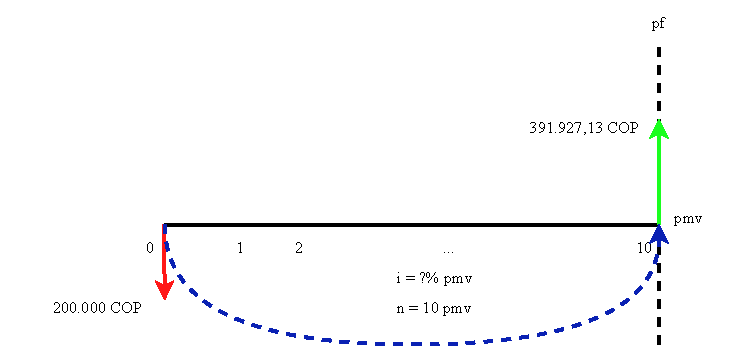
\includegraphics[scale=1]{ejemplos/3/Graf3Ej3Cap11.pdf} }
		\\
		\multicolumn{3}{|c|}{$391\text{.}927,13 COP =  200\text{.}000 COP(1+i)^{10}$}
		\\
		\multicolumn{3}{|c|}{$ i=TIRM(A)=6.96\% pmv$}
		\\
		\multicolumn{3}{|c|}{$ \text{TIRM(B):  Trasladamos a valor final la serie de 10 ingresos de 16.280 COP y tenemos:} $}
		\\
		\multicolumn{3}{|c|}{$ 16\text{.}280 COP(\frac{(1+0.05)^{10}-1}{0.05}) = 204\text{.}768,1 COP  \textbf{    Ecuación de equivalencia }$}
		\\
		\multicolumn{3}{|c|}{ 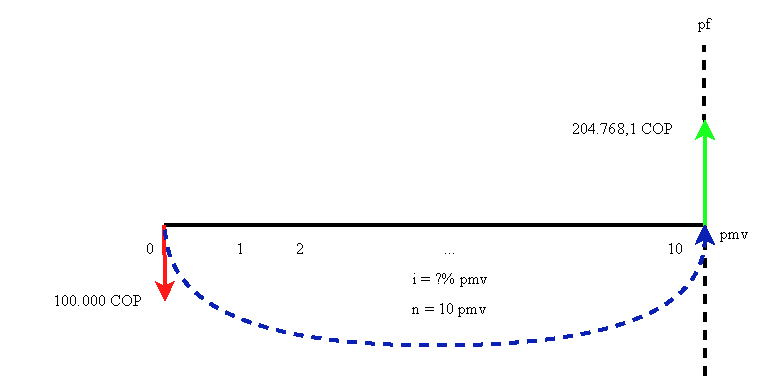
\includegraphics[scale=1]{ejemplos/3/Graf4Ej3Cap11.pdf} }
		\\
		\multicolumn{3}{|c|}{$ 204\text{.}768,1 COP = 100\text{.}000 COP(1+i)^{10}$}
		\\
		\multicolumn{3}{|c|}{$i=TIRM(B)=7.43\% pmv$}
		\\
		\multicolumn{3}{|c|}{$\text{Se concluye que TIRM(B) es mejor que TIRM(A)}$}
		\\
		\multicolumn{3}{|c|}{$\text{Como el proyecto A es más costoso que el proyecto B }$}
		\\
		\multicolumn{3}{|c|}{$\text{debemos adicionar al proyecto B  el proyecto adicional con inversión inicial de 100.000 COP y }$}
		\\
		\multicolumn{3}{|c|}{$\text{lo evaluaremos a la tasa del 5\% pmv.}$}
		\\
		\multicolumn{3}{|c|}{$ 100\text{.}000 COP(1+0.05)^{10} = 162\text{.}889,46 COP$}
		\\
		\multicolumn{3}{|c|}{ 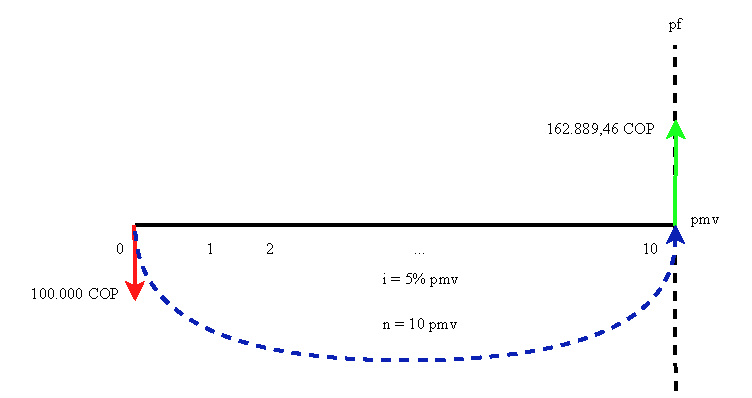
\includegraphics[scale=1]{ejemplos/3/Graf5Ej3Cap11.pdf} }
		\\
		\multicolumn{3}{|c|}{$\text{Entonces el nuevo proyecto B quedará formado por el proyecto B incial   }$}
		\\
		\multicolumn{3}{|c|}{$\text{más el proyecto adicional con el siguiente flujo de caja:  }$}
		\\
		\multicolumn{3}{|c|}{$\textbf{Ingresos en el periodo 10: } 204\text{.}768,1 COP + 162\text{.}889,46 COP = 367\text{.}657,56 COP$}
		\\
		\multicolumn{3}{|c|}{$\textbf{Costo inicial: } 100\text{.}000 COP + 100\text{.}000 COP = 200\text{.}000 COP$}
		\\
		\multicolumn{3}{|c|}{ 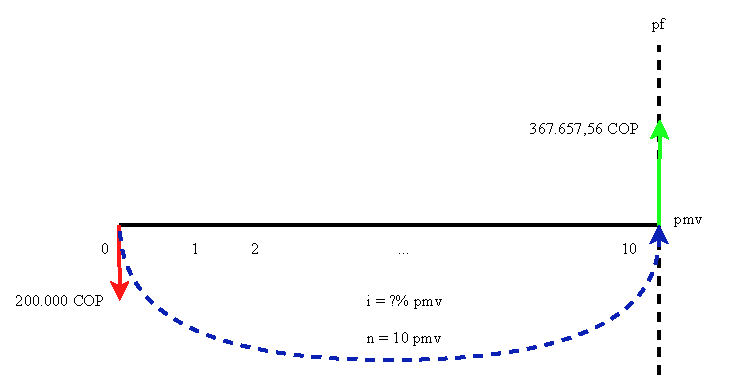
\includegraphics[scale=1]{ejemplos/3/Graf6Ej3Cap11.pdf} }
		\\
		\multicolumn{3}{|c|}{$\text{ Ahora calculamos la TIR de este nuevo proyecto así: } $}
		\\
		\multicolumn{3}{|c|}{$367\text{.}657,56 COP = 200\text{.}000 COP(1+i)^{10}$}
		\\
		\multicolumn{3}{|c|}{ \text{Al despejar se tiene que i = TIR(B) = 6,28\% pmv, el cual es inferior a la TIR(A)}}
		\\
		\hline

		%%%%%%%%%% FIN MATEMÁTICAS
		%%%%%% FIN DESARROLLO MATEMÁTICO
		%%%%%% INICIO RESPUESTA
		\rowcolor[HTML]{FFB183}
		%%%%%%%%%%INICIO TITULO
		\multicolumn{3}{|c|}{\cellcolor[HTML]{FFB183}\textbf{6. Respuesta}}                                                                           \\ \hline
		%%%%%%%%%% FIN TITULO
		%%%%%%%%%% INICIO RESPUESTA MATEMÁTICA

		\multicolumn{3}{|c|}{ \text{Es mejor invertir en el proyecto A que en el proyecto B, ya que la TIR y }}
		\\
		\multicolumn{3}{|c|}{ \text{VPN del proyecto A son mayores que la TIR y VPN del proyecto B respectivamente.}}
		\\
		\hline


		%%%%%%%%%% FIN MATEMÁTICAS
		%%%%%% FIN RESPUESTA
	\end{longtable}
	%Se crean dos lineas en blanco para que no quede el siguiente texto tan pegado
	%\newline \newline %USARLO SI CREES QUE ES NECESARIO
\end{center}
%%%%%%%%%%%%%%%%%%%%%%%%%%FIN EJERCICIO 1 %%%%%%%%%%%%%%%%%%%%%%%%%%%